\chapter{Future work}
This PhD provides a snapshot of research I have done in recent years. This work fits within a larger body of research with similar overall objectives, to improve both the software and how that software is developed. This chapter introduces various topics related to my ongoing research which may be of interest to the research community.

\section{Further evaluation of Analytics tools}

With discovering the many and various flaws and quirks in Google's analytics products I decided a set of experiments would help increase the trust and transparency of Android Vitals and Google Play Console. Aspects of these experiments may also be highly relevant to evaluate other analytics tools, products, and services. 

Testing and evaluation of third-party commercial services involves awareness and compliance with ethical aspects and various legal terms and conditions. Some of the experiments could trigger defensive mechanisms used to 'protect' large-scale online services such as Google Play. For instance App Stores, including Google Play, are known to take protective and corrective activities related to fake reviews. Some experiments might want to assess the effectiveness of protective defenses, others may aim to avoid triggering them. 

Google is known to take punitive actions against developers whom it deems to be related to undesirable behaviours. 
%MUST-DO add references to examples. 
As various people have discovered to their cost, the service provider may choose to disable access and remove all the apps in Google Play that are deemed - by Google - to be associated with an individual.\citep{Martinez_2019}. Google also blocked developers and their apps not for what \emph{that} developer did, but for what Google decided were infringements by people 'associated' with the developer. This has caused businesses to fold where Android apps were their route to market\citep{Martinez_2019, mark_dodson_medium_story}. We, therefore, restricted our testing, in order to minimise the risk of the apps being blocked. This was to protect the projects who have worked with us, and their apps, otherwise we risk inadvertently blocking apps for a user population of approximately 500,000 users and also the developers of those apps. Google acts as both judge and jury. There has been successful and effective research into the contents of an app store, and Google Play in particular where the researchers successfully circumvented various protection mechanisms in \textbf{YYYY}, 
% MUST-DO add year, ideally add additional examples
their research was read-only and able to be scaled out. Research into the analytical tools and reporting requires the developers to identify themselves, pay a fee, and also their activity is tracked to their account. Also there needs to be usage of the apps which is another consideration that would need to be addressed. These constraints and factors indicate previous approaches may be counter-productive and block the research, the researchers, and potentially apps, organisations, and people, related to the researchers:~\emph{caveat investigator!}



We have requested clarification from Google on what testing would be appropriate, they have yet to provide any specific answers beyond \emph{"whilst we understand that your testing is designed to learn more about how our products work, we cannot treat your app any differently to the others on the store. Our normal policies and mechanisms apply."} They also referred us to the Policy Center, which states \emph{"We don’t allow apps that crash, force close, freeze, or otherwise function abnormally."}~\citep{google_play_policy_center_broken_functionality}. We are in ongoing discussions with the relevant engineering teams at Google to obtain clarification.

Note: In terms of ethical aspects and disclosure, the author read and reviewed various legal materials published by Google for the service being evaluated, including the Google Play Developer Policy Center\citep{google_play_developer_policy_center}, and the Distribution Agreement\citep{google_play_developer_distribution_agreement}. The author has also reported the various issues found with the product and engineering team at Google.




As these actions can include a lifetime ban for the account deemed to have transgressed, and for other accounts it considers are related, the effects of their actions can be far reaching and remove all revenues for an organisation's Android apps where the onus is on the people in that organisation being able to convince Google of the merits of reinstatement often without knowing what the reasons were, what the evidence was, and with no other practical way of restoring their account.

The Google Engineering team have been defensive and guarded in terms of suggestions to help evaluate the behaviours of their system. SHOULD-DO add some examples. 

A cautious set of basic tests to help establish characteristics of analytics from no (zero) to tens of users is available online at 
\url{https://joedocs.com/julianharty/evaluating-gpc-reports}

\textbf{Placeholders to extend on this topic}: Holding ourselves and each other to account. Humility, openness, comparisons with financial auditing of businesses. \emph{c.f.} Sentry.io's work, opensourcing of client libraries, etc. 

\begin{itemize}
    \item Due diligence. \emph{`Trust and Confirm')~\footnote{\url{https://www.leadergrow.com/articles/443-trust-but-verify}}}. The risks of overtrusting and not doing due diligence, especially where money is involved. The author encourages verification (as I do). Beware of end to end systems that are not verifiable by an outside party~\footnote{\url{https://www.forbes.com/sites/frankarmstrong/2019/10/21/trust-but-verify/}}.
    \item \emph{``The Only Thing Necessary for the Triumph of Evil is that Good Men Do Nothing"}~\footnote{\url{https://quoteinvestigator.com/2010/12/04/good-men-do/}}
\end{itemize}

\section{Research into Google Android data collection}
The mechanism(s) Google uses to collect data on devices is worthy of research given the scope, range and effects of this data in terms of assessing qualities of all the Android apps in Google Play.

My work has identified numerous flaws in the reporting, do any of these stem from the data collection on the devices? Is it possible? is it practical? to generate fake data that Google would use and rely on? Research has already found evidence of systemic tainting of ratings and reviews, perhaps it's also possible that diagnostic and usage data can also be tainted at scale?

related work: Botnets, black market reviews, device farms using emulators, device farms intended for testing, ...

A related topic is to better understand whether the underlying device data can be accessed using non-Google software. 

\begin{enumerate}
    \item What data does Android Vitals capture?
    \item Where is that data available on Android devices?
    \item Ways to access that data?
    \item Homebrew approach to accessing, collecting, and analysing the data.
\end{enumerate}

\subsection{Homebrew}
As discussed in section \href{platform-level-analytics}{\emph{\nameref{platform-level-analytics}}}, parsing the Android logs requires Android permission(s) ... Once the software has been granted permission it can read all the logs (...) and parse them. [Presumably] the logs are read-only for apps (the history can be cleared using the \texttt{adb logcat} command-line command externally (e.g. from a PC).

Structure and presentation of content in the Android logs: ...
Consistency in pertinent events in Android logs (we believe they're consistently formatted with predictable elements always provided, which makes them easier to parse and process).



\section{Comparing static-analysis warnings with failures reported in usage analytics}
As the research of~\citep{khalid2016_examining_the_relationship_between_findbugs_warnings_and_app_ratings} found, there were correlations between static analysis warnings for poorly rated apps for three categories of warnings: 1) bad practice, 2) internationalization, and 3) performance. The first and third of these categories are also provided by various analytics tools including Android Vitals. Therefore it may be of interest to research whether there are correlations between static-analysis warnings for these categories and the crash and ANR clusters reported in the appropriate tools. 

The results of these comparisons may help in several areas of further research:
\begin{enumerate}
    \item Warnings are reported by static-analysis tools but not reported in the analytics tools,
    \item failures in the field are also detected by static-analysis tools, and
    \item failures in the field are not detected by static-analysis tools.
\end{enumerate}

In each case there is the potential to investigate the effects. Here are some suggestions:
\begin{enumerate}
    \item Perhaps the code-paths in the app are not used in practice in the field. If so, there may be usability and/or reachability issues. Developers can then take corrective action or remove the code if they decide it is not productive and reduce the size and complexity of the app.
    \item If the same faults are detected in both tools, potentially developers could find and fix the issues before the software is released. These fixes may improve the reliability of the app in practice and increase the potential for the app to succeed in terms of app store quality ratings and promotion by the app store as well as also improving the end user experience.
    \item Where failures are only found when the software is used, could static analysis be enhanced to find some or all of these faults sooner?
\end{enumerate}

\section{Enhancing quality vs. enhancing UX}\label{enhancing-quality-vs-enhancing-ux}
Success of software is multifactorial and development teams need to consider where, when and how to focus their energies to achieve satisfactory outcomes for themselves and their patrons (often their management and funders). Where does improving and achieving high-quality software fit amongst other demands on their time and energies?

\begin{figure}[htbp!]
    \centering
    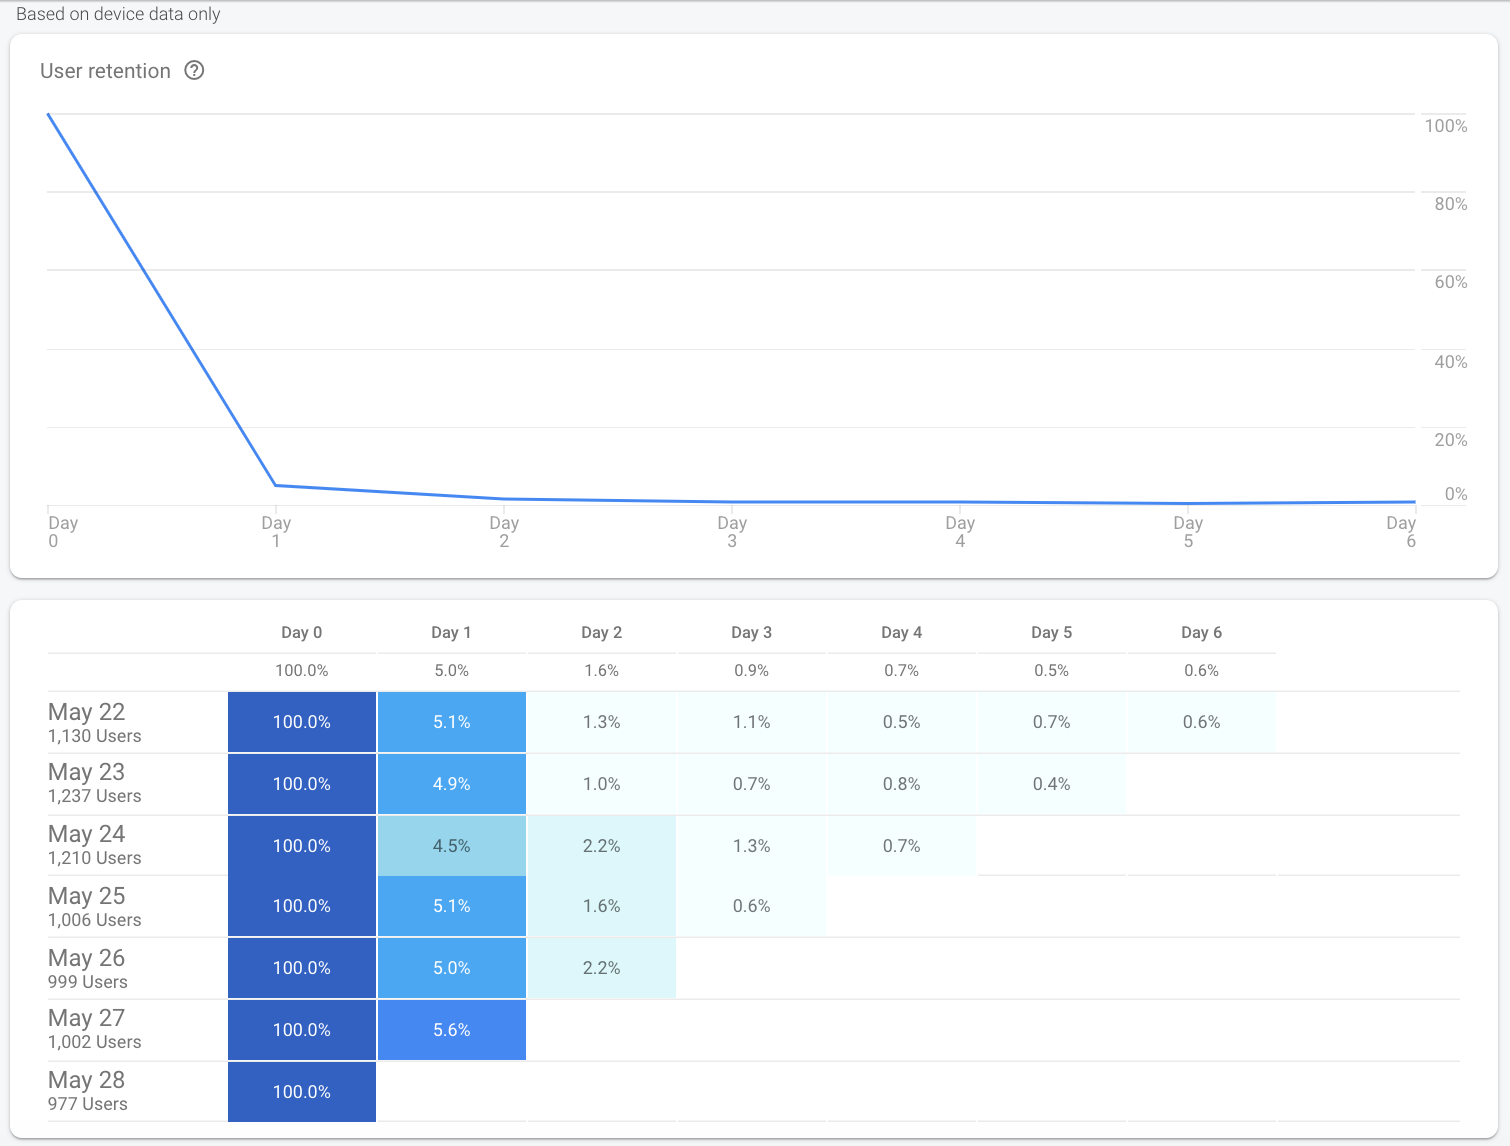
\includegraphics[width=10cm]{images/firebase/Firebase-pocketcode-android-7-day-new-user-retention-29-may-2020.png}
    \caption{Firebase>Catrobat>New User Retention}
    \label{fig:Firebase-pocketcode-android-7-day-new-user-retention-29-may-2020}
\end{figure}

An area of my ongoing research is to evaluate the impacts of enhancing software quality in terms of stability compared to enhancing the UX of an app. The Pocket Code mobile Android app has low retention rates for new users according to Firebase, the 7 day retention of new users is illustrated in Figure \ref{fig:Firebase-pocketcode-android-7-day-new-user-retention-29-may-2020}. Both the iOS and Android Pocket Code apps have similar screens, especially the initial screens seen by new users of either app. Through our research and the focus on identifying and fixing various stability metrics we plan to focus on improving the design of the user experience for new users. One measure will be the `new user retention' report.

There has been some small scale research, involving 12 university students, that provided the authors with useful insights into designing onboarding tasks for mobile apps~\citep{strahm2018_mobile_app_onboarding}. Their approach may yet be useful and relevant as part of enhancing UX for new users of apps, including Pocket Code.

\begin{figure}[htbp!]
    \centering
    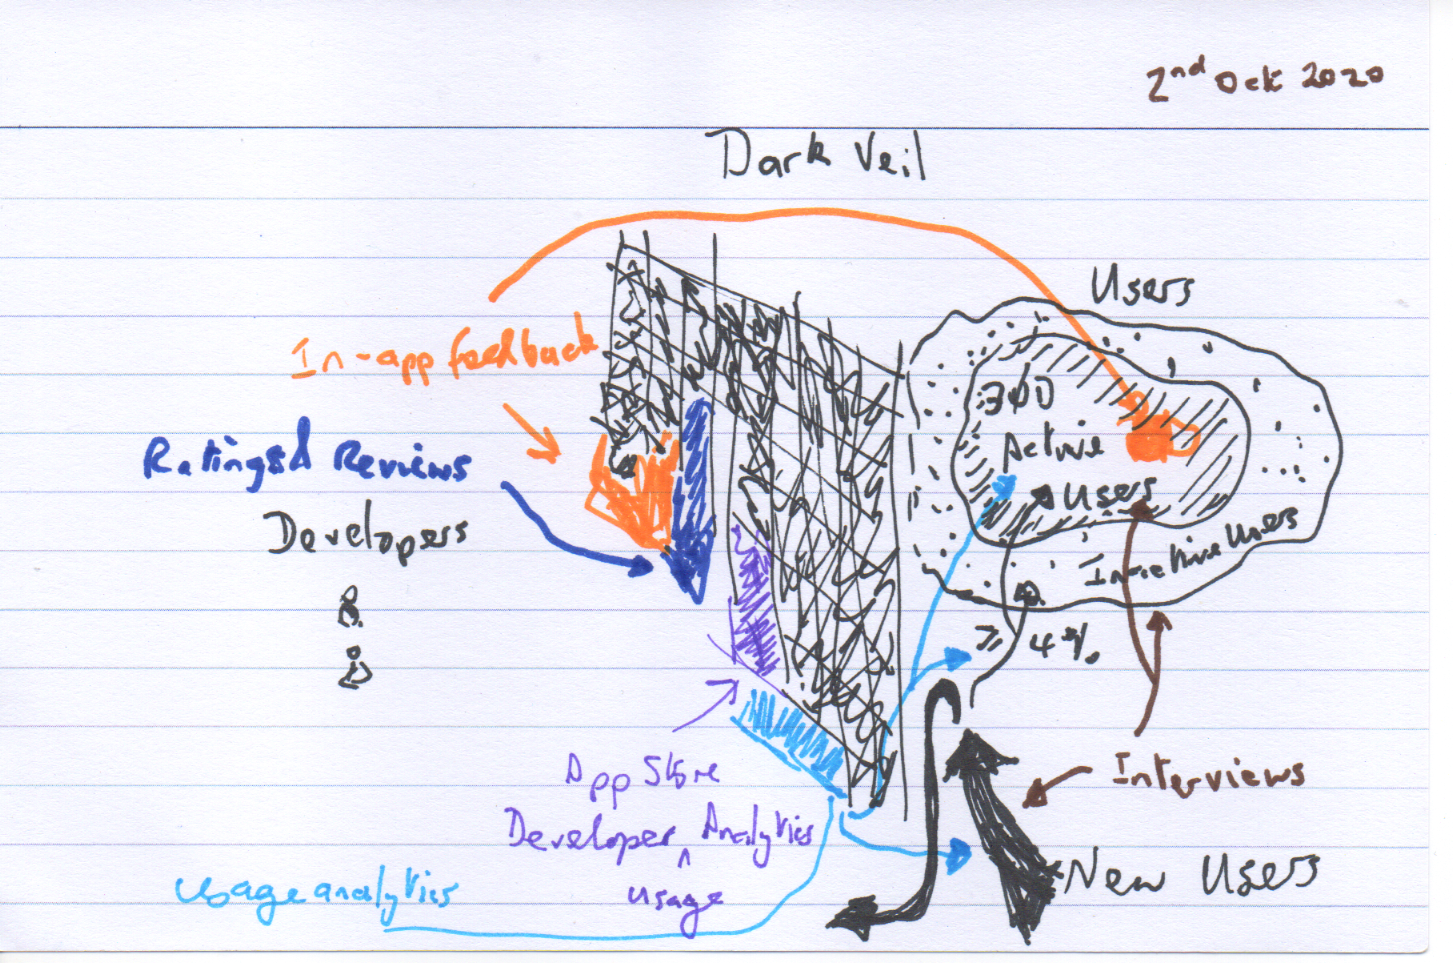
\includegraphics[width=13cm]{images/rough-sketches/sources-of-information-with-app-store-1.png}
    \caption{Sources of information with an App Store}
    \label{fig:sources-of-info-with-app-store-future-work-ch}
\end{figure}

As Figure~\ref{fig:sources-of-info-with-app-store-future-work-ch}~\footnote{Figure reproduced from Figure~\ref{fig:sources-of-info-with-app-store-background-ch} in an earlier chapter for a better reader experience.} illustrates there are various sources of information, the app store is one of four main routes to provide information (the others are: in-app feedback, other forms of feedback, and in-app analytics).

\section{Privacy-centric analytics in mobile apps}
There has been some work and research into specific areas of privacy, such as the consideration of PII data collection where some analytics providers tell developers not to collect or process PII data, however there's been little checking or enforcement in the industry at large. A startup, Iteratively~\citep{iteratively_homepage}, is an organisation working to improve the practices around several aspects of privacy in terms of the data that is collected and where and how the data is processed.

TBC - discuss my work and - security layers, rings, data-plane, data-locality, federated analytics processing.

\section{Developer-centric logging and analytics in mobile apps}
Developers use logging for various reasons when they work with source code. Therefore developers use logging when they work on source code for mobile apps. Do they use logging in particular ways or for specific purposes when developing mobile apps? Research considerations include the use of remote logging and/or the use of mobile analytics.

My research in mobile analytics overlaps and closely aligns with research on logging - both are used by software development teams to learn about how their software behaves. I am part of a group of distributed, international researchers investigating aspects of how and why developers add logging to their mobile applications. One of our current research areas investigates the use of Google Firebase Analytics for logging. \emph{Ad-hoc} research notes are available at \url{https://joedocs.com/julianharty/apm-logging-research}.


\section{Improving the design, implementation and engineering of in-app analytics}
Research in approaches to improve the design, implementation and engineering of in-app analytics may inform the state of the art in the use of in-app analytics, particularly for software engineering and software quality. It may also help inform and guide the practice of in-app analytics. 

Commercial services, such as \href{http://iterative.ly}{Iteratively}, aim to facilitate the \emph{``capture [of] accurate analytics right firs time"} and enable developers to \emph{``Quickly instrument analytics with code snippets and automated QA."} through their software tools. How might services such as these help development teams improve their engineering of in-app analytics? 

Two suggested areas of research are whether these tools successfully guide developers to:
\begingroup
\renewcommand{\theenumi}{\alph{enumi}}
\begin{enumerate}
    \item actively use data already available to them?
    \item design how to use optional analytics tools efficaciously?
\end{enumerate}
\endgroup
% Thanks to: https://tex.stackexchange.com/questions/346787/how-can-i-get-a-list-starting-with-a-b-c-instead-of-1-2-3


\subsection{Adding in-app analytics to PocketCode}
PocketCode has been subject to active and ongoing practical research for several years and the app and surrounding ecosystem is rich and mature. The software and materials are opensource and intended to be used for research therefore it is a viable candidate for researching in-app analytics.

The Pocket Code Android app included the legacy Fabric Crashlytics analytics library for several years predating my involvement with the project (the earliest commit to add Fabric Crashlytics is on \nth{27} June 2017~\footnote{\href{https://github.com/Catrobat/Catroid/commit/95aa37ff5263402b41b63f50296aabc8c354433e}{\texttt{CAT-2420 Replace Firebase with Crashlytics}}}). This recorded both caught and uncaught exceptions but nothing else about how the app was used, or by whom. As part of my collaboration with the Catrobat team we agreed we would design and add in-app analytics in addition to the crash reporting. This work coincided with migrating from the legacy Fabric reports to the replacement Firebase reports so Firebase Analytics was selected. I helped lead the initial design and testing of the in-app analytics~\footnote{Various details are available in a Google hosted document~\url{https://docs.google.com/document/d/1cqCP2aqcx8mpTTHWe9ooGygtXh7eTvYzM3f9FbexUNM/edit?usp=sharing}}. The work has been delayed because of various impacts of the COVID-19 pandemic, the aim is to resume it as various countries and regions emerge from their respective lockdowns.


\section{Dynamic, adaptive logging in mobile apps}
This is a placeholder and a reminder to incorporate some early ideas on this topic in an unpublished paper titled \emph{``Dynamic Distributed Logging and Analytics"}, see \url{https://www.overleaf.com/read/mgcrcqkbsnzh}.



\section{Using mobile analytics to improve testing of mobile apps}
% MUST-DO expand this section.
\begin{itemize}
    \item Using Mobile Analytics to improve the testing of mobile apps. This was work I had hoped to perform as part of this research, various practical constraints meant this was not practical during the PhD.
\end{itemize}

\begin{figure}[!htbp]
    \centering
    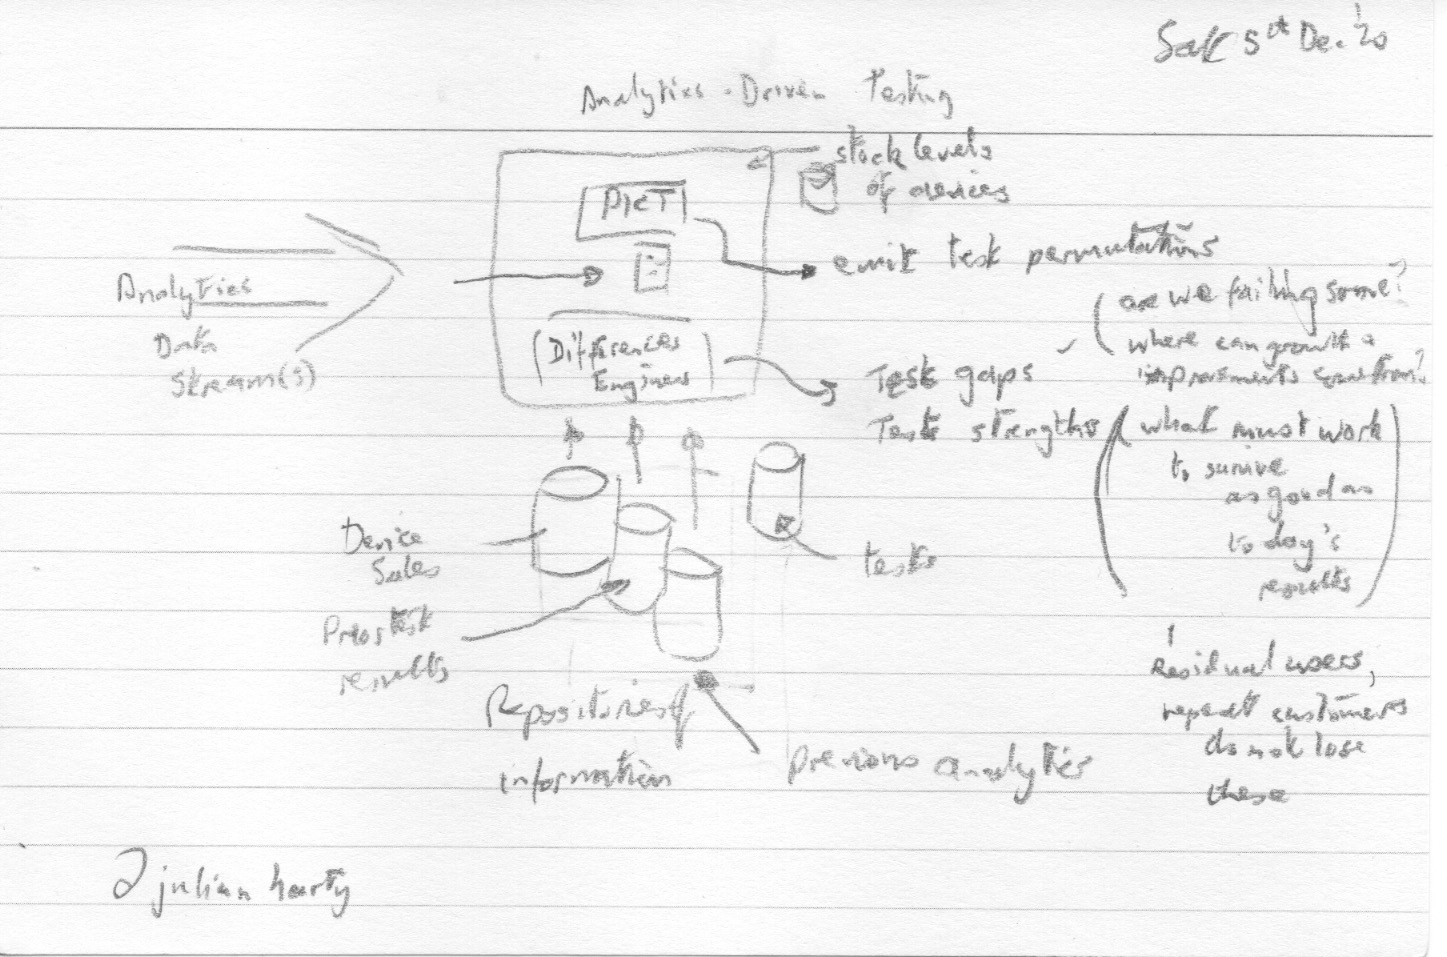
\includegraphics[width=\textwidth]{images/rough-sketches/Analytics-driven-testing-including-PICT.jpeg}
    \caption{Analytics-driven testing}
    \label{fig:roughsketch:analytics-driven-testing-incl-PICT}
\end{figure}

The approach consists of various categories of data, some changing quickly and intended to be the main impetus (the analytics data streams), some changing slowly (various repositories of industry data, prior test results, previous analytics for our system, and known tests suitable for our system). There may also be stock levels of available resources for testing e.g. unused devices in a device farm.
Tools including Microsoft PICT (as a working example) can combine the data to emit test cases (or test permutations) that a candidates to be executed. These can be executed through a combination of humans and/or automation. 

At least two categories of tests to devise:
\begin{enumerate}
    \item test gaps – if there are dips in the actual analytics patterns compared to what we’d predict / expect? if so, test into these areas to see if there are problems in the real-world we’d like to try addressing. This may include areas where we can grow the usage and userbase, etc.
    \item test strengths – where the tests are designed to ensure we do not make things worse for our current userbase and their use of the software. There are similarities with businesses wanting to ensure they retain repeat business, residual profitable/desirable users, and so on.
\end{enumerate}

A proof-of-concept for analytics driven testing: 


\begin{itemize}
    \item Use single-digit data permutations
    \item Use one to a few of the available categories of data e.g. Android releases, device models, locale and create a PICT configuration file based on several distinct snapshots of these inputs of permutations.
    \item Test Strengths testing:
    \begin{itemize}
        \item Execute tests based on the output of PICT
        \item Do mainly manual testing
        \item Collect analytics results using the same tools (where practical) that provided the production analytics. Compare the patterns of the analytics from the testing to those from the production snapshots.
    \end{itemize}
    \item Test Gaps testing:
    \begin{itemize}
        \item Provide several data sets of predicted usage volumes.
        \item Perform differences analysis to compare representative patterns in the analytics with these data sets.
        \item See if performing the differences accurately determines troughs in the analytics data (where usage is materially less than predicted) and emit test permutations to probe the system to establish whether the system works well for users on those permutations.
    \end{itemize}

\end{itemize}
 


\section{Digital twins for software apps}
Digital twins are variously defined as \emph{``a high-fidelity digital model of a physical system or asset that can be used e.g. to optimize operations and predict faults of the physical system."}~\citep{pokhrel2020_digitaltwin_for_cybersecurity} and \emph{``Digital twins integrate IoT, artificial intelligence, machine learning and software analytics with spatial network graphs"}~\citep{wikipedia__digital_twin} (attributed to Microsoft in 2018 in the Wikipedia article). Twins have been used for various engineering challenges including jet turbine performance engineering and may help transform the engineering lifecycle for many products, including jet turbines~\citep{read2018_digital_takeover_avionics}, cars. As~\citep{pokhrel2020_digitaltwin_for_cybersecurity} observes, digital twins may also represent cyber-security and potentially humble, mobile apps.

``A Digital Twin will continuously learn and update itself using data from sensors that monitor various aspects of the real-life product’s environment and operating conditions. It can also factor in historical data from prior usage."~\url{https://www.rolls-royce.com/media/our-stories/discover/2019/how-digital-twin-technology-can-enhance-aviation.aspx}
% https://www.aerospacetechreview.com/twinning-digital-twins-show-their-power-by-louise-bonnar/

A digital twin for mobile apps is likely to include controlled run-time environments including high-fidelity emulators and physical devices since some problems and behaviours may be triggered and/or exposed by particular run-time environment. Mobile Analytics may help inform the selection of run-time environment as well as the identification of software quality concerns. As mobile apps are increasingly used in very sensitive and critical environments where the consequences are material, digital twins may also be used to validate the behaviours and outputs of the apps for end users.

% https://golden.com/wiki/Digital_twin-6MX6WP % repeats the definition from Wikipedia that apparently came from MSFT in 2018.


\section{Finding usage failures pre-release}
Learning about issues, including failures, when the software is in-use is useful and enables developers to address them in subsequent releases. However there may be effective ways to find at least some of these issues \textit{before} the software is released. Hypothetically, static analysis and other code quality tools could find some or even many of the issues. If so, what would the value be to developers in using those tools to find these issues? what are the preceived costs? As research indicates, developers don't use static analysis tools [much] 
\textbf{MUST-DO} cite the Google Research paper on this topic.

ON a related note, a failure is specific yet may represent a class of similar flaws in a codebase and even in similar codebases. 
% From Oliveria...
% Understanding if and when Android abstractions cause programs to fail, in particular due to uncaught exceptions, can make developers use them in a more disciplined way. It raises awareness for the need for catalogs of exception handling bug patterns (Coelho et al., 2011) and bug hazards (Coelho et al., 2015), as well as best practices. Moreover, it can influence code review activities, since code reviewers will know where to look for a common source of potential bugs, for example, calls to the get method of class AsyncTask for which there is no handler. Testers can also leverage this knowledge to create specific tests for common error conditions related to these abstractions. Tool developers can augment their bug finding tools to look for unprotected uses of these abstractions, e.g., activities that run in a GUI thread that has no associated UncaughtExceptionHandler.
% and: 
% The expected outcome is a list of typical bug patterns made when using Android abstractions. Based on those findings, we intend to document them in the form of cookbooks with best Android practices. 

\section{Summary of Future Work}
The thesis is a snapshot of work done to date. The PhD journey and a combination of the relationships and experiences that have been established on the journey have led to various interesting and related areas of ongoing and future work which I am actively engaged in. Please get in contact if you would like to collaborate with any of these and/or with other topics that relate to my research.
